\section{Zielsetzung}
\label{sec:Zielsetzung}
In diesem Versuch wird das Trägheitsmoment verschiedener
geometrischer Körper bestimmt und der Steiner'sche Satz bestätigt.



\section{Theorie}
\label{sec:Theorie}

Das Trägheitsmoment $I$ ist eine Größe, die zur Charakterisierung
der Dynamik von Drehbewegungen benutzt wird. Für eine
punktförmige Masse $m$, die sich im Abstand $r$ zu einer festen
Rotationsachse aufhält, ergibt sich für dieses
\begin{equation}
I = mr^2.
\end{equation}
Das Gesamtträgheitsmoment ausgedehnter Körper setzt sich aus den
Einzelträgheitsmomenten der Masseelemente $m_{\text{i}}$,
welche sich im Abstand $r_{\text{i}}$ zur Drehachse aufhalten,
zusammen. Somit gilt für das Gesamtträgheitsmoment:
\begin{equation}
I = \sum_{\text{i}} r_{\text{i}}^2 \cdot m_{\text{i}}
\end{equation}
Für infinitisimale Massen $dm$ ergibt sich folglich
\begin{equation}
I = \int r^2 dm.
\end{equation}
Die Trägheitsmomente einiger geometrischer Körper sind Abb.1 zu
entnehmen.
\begin{figure}[H]
\centering
\caption{Trägheitsmomente geometrischer Körper. [1]}
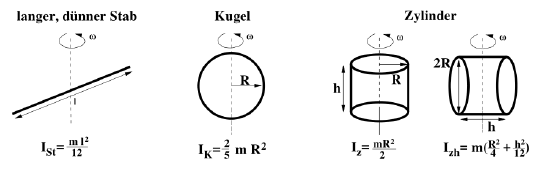
\includegraphics[scale=1]{koerper.PNG}
\label{fig:koerper}
\end{figure}
Die bisher genannten Fälle beziehen sich auf Rotationsbewegungen,
bei denen die Rotationsachse durch die Schwerpunktachse des
Körpers verläuft. Ist dies nicht gegeben, so berechnet sich
das Trägheitsmoment mit Hilfe des Steiner'schen Satzes:
\begin{equation*}
I = I_{\text{s}} + m \cdot a^2,
\end{equation*}
wobei $I_{\text{s}}$ das Trägheitsmoment bezüglich der
Schwerpunktachse und $a$ der Abstand der
tatsächlichen Drehachse zu dieser ist.
\par
Wenn auf einen drehbaren Körper die Kraft $\vec{F}$ im Abstand
$\vec{r}$ der Achse wirkt, so wirkt auf ihn ein Drehmoment
$\vec{M}$
\begin{equation}
\vec{M} = \vec{F} \times \vec{r}.
\end{equation}
Wirkt dem Körper, welcher um den Winkel $\phi$ ausgelenkt wird,
ein rücktreibendes Drehmoment, beispielsweise durch eine Feder,
entgegen, so handelt es sich um ein schwingendes System, welches
harmonische Oszillationen ausführt. Die Periodendauer $T$ ist dabei
\begin{equation}
T = 2\pi \sqrt{\frac{I}{D}}.
\label{eqn:Periodendauer}
\end{equation}
Hierbei stellt $D$ die Winkelrichtgröße dar. Sie steht mit
dem Drehmoment $M$ über
\begin{equation}
M = D \cdot \phi
\end{equation}
in Verbindung. Das System führt nur für kleine
Drehwinkel $\phi$ \(\ll\) 5° harmonische Schwingungen aus.
\par
Die Winkelrichtgröße $D$ kann statisch durch Messen der Kraft
senkrecht zum Radius bei Auslenkung um den Winkel $\phi$
bestimmt werden:
\begin{equation}
\label{eqn:winkelrichtgroeße}
D = \frac{F \cdot r}{\phi}.
\end{equation}
Bei dynamischen Messungen wird das System zu harmonischen
Schwingungen angeregt. Aus Gl. \eqref{eqn:Periodendauer} folgt
\begin{equation*}
I = \frac{T^2D}{4\pi^2},
\end{equation*}
wobei $I$ nun das gesamte Trägheitsmoment darstellt. Um das
Trägheitsmoment $I_{\text{K}}$ des Rotationskörpers zu erhalten,
muss noch das Trägheitsmoment $I_{\text{D}}$ der Drillachse
subtrahiert werden:
\begin{equation}
  \label{eqn:taegheitsmoment}
I_{\text{Körper}} = \frac{T^2D}{4\pi^2} - I_{\text{D}}.
\end{equation}